\documentclass[12pt]{article}

\usepackage[utf8]{inputenc}
\usepackage[portuguese]{babel}
\usepackage{sbc-template}

\usepackage{graphicx,url}

\usepackage{float}

% Exemplo de enumeracao
%\begin{enumerate}
%	\item Item1
%	\item Item2
%	\item Item3
%\end{enumerate}

% Exemplo de figura
%\begin{figure}[ht]
%\centering
%\includegraphics[width=.9\textwidth]{arquivo.eps}
%\caption{Legenda}
%\label{fig:label_da_figura}
%\end{figure}

% Exemplo de código
% \verb|classe.metodo()|
     
\sloppy

\title{Projeto MyMon3y}

\author{Jaindson Valentim\inst{1}, Matheus Gaudencio\inst{1}}

\address{DSC -- Universidade Federal de Campina Grande
  (UFCG)\\
  Av. Aprígio Veloso, 882 -- Bl. CN -- Campina Grande -- PB -- Brazil
  \email{\{jaindsonvs, matheusgr\}@gmail.com}
}

\begin{document} 

\maketitle

\begin{resumo}
Este relatório técnico descreve o processo de desenvolvimento, a arquitetura e as tecnologias de apoio utilizadas na construção do projeto da disciplina ``'Projeto de Software Orientado a Objeto'' oferecida no período 2009.1 e ministrada pelo professor Dr. Jacques Philippe Sauvé.
\end{resumo}

\section{Introdução}
\label{intro}

Como parte das atividades da disciplina ``Projeto de Software Orientado a Objeto'' oferecida no período 2009.1 e ministrada pelo professor Dr. Jacques Philippe Sauvé, pediu-se um sistema de controle de finanças pessoais, o \textit{MyMoney} (implementado com o nome de \textit{MyMon3y} pelos desenvolvedores). Este relatório descreve a construção dos dois primeiros \textit{milestones} do projeto: a definição das \textit{User-Stories} e a codificação da lógica de negócio.

Este documento está estruturado da seguinte forma: a seção~\ref{especificacao} apresenta a especificação do projeto, descrevendo as \textit{User-Stories} planejadas e o modelo lógico de dados. Em seguida, a seção~\ref{arquitetura} mostra a arquitetura do software. Por fim, na seção~\ref{tecnologias}, são descritas as tecnologias utilizadas na implementação do sistema.

\section{Especificação}
\label{especificacao}

A especificação inicial foi fornecida pelo cliente do sistema (professor Dr. Jacques Philippe Sauvé) através do seguinte parágrafo:

\begin{quote}
MyMoney é um sistema de controle de finanças pessoais onde \textbf{gastos e entradas} de dinheiro podem ser \textbf{registrados e classificados} e \textbf{relatórios} podem ser \textbf{gerados}. Há um \textbf{mecanismo de notificação de contas a pagar} e \textbf{mecanismos de importação de dados} de arquivos gerados como extratos do banco.
\end{quote}

A marcação em negrito foi realizada pelos desenvolvedores deste sistema, e denota os elementos mais importantes extraídos da especificação. Tais elementos norteiam a definição das funcionalidades gerais do sistema:
    
\begin{itemize}
 \item Registro de gastos e entradas de dinheiro (transações)
 \item Registro das transações por categorias
 \item Impressão de relatórios
 \item Notificação de pagamentos
 \item Importação de dados de extratos bancários
\end{itemize}

A partir da especificação, são definidos: o modelo lógico de dados (subseção~\ref{modelo}) e as \textit{User-Stories} (subseção~\ref{us}).

\subsection{Modelo Lógico de Dados}
\label{modelo}

Foram definidas como entidades do modelo lógico de dados:

\begin{description}
 \item [Usuário] Representa a conta de um usuário com os atributos \textit{login} (o email do usuário) e \textit{senha}. Cada usuário dispõe de diversas \textit{categorias} onde \textit{transações} podem ser cadastradas.
 \item [Categoria] Uma \textit{categoria} agrupa transações de um determinado usuário.
 \item [Transação] \textit{Transação} representa uma movimentação financeira realizada pelo usuário. Apresenta uma breve \textit{descrição}, a \textit{data}, \textit{comentário} e o \textit{valor} da transação. Uma movimentação financeira de gasto ou entrada é indentificada pelo atributo \textit{booleano} \textit{crédito}, e há um atributo que descreve a \textit{data de aviso prévio}, ou seja, a data em que uma notificação deve ser enviada ao usuário.
\end{description}

Estas são as entidades persistidas em que o sistema opera toda lógica de negócio. A apresentação da composição das entidades pode ser vista na figura~\ref{modelo-fig}.

\begin{figure}[H]
\centering
  \label{modelo-fig}
  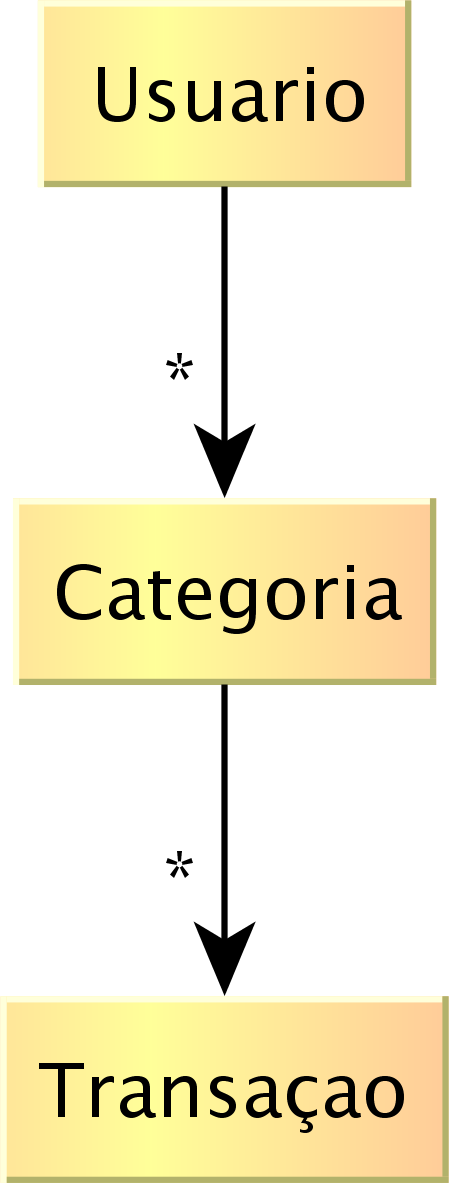
\includegraphics[scale=0.1, bb=0 0 449 1183]{./modelo.png}
  % modelo.png: 449x1183 pixel, 72dpi, 15.84x41.73 cm, bb=0 0 449 1183
  \caption{Modelo lógico de dados}
\end{figure}

O sistema ainda faz uso de uma entidade não persistente: \textbf{relatório}. Cada \textbf{relatório} representa uma agregação de \textbf{transações} de determinado \textbf{usuário} e existe apenas durante a operação de emissão de relatório.

\subsection{User-Stories}
\label{us}

Usando a especificação e as mensagens trocadas em lista e em avisos em sala-de-aula, foram definidas 8 \textbf{User-Stories} descritas à seguir. As \textbf{User-Stories} que trabalham alterando elementos do modelo lógico de dados apresentam também uma \textbf{User-Story} responsável pela funcionalidade da persistência de tais alterações.

Cada \textbf{User-Story} é especificada através dos seguintes elementos:
\begin{description}
 \item [Descrição] Pequena descrição do caso de uso.
 \item [Entidade] Entidades do modelo de dados que são criadas, atualizadas ou removidas pela \textit{User-Story}.
 \item [Persistência] Determina se há ou não necessidade do tratamento de persistência das alterações realizadas no modelo de dados.
\end{description}

\subsubsection{User Story 1 - Criação/edição de Conta}

\begin{description}
 \item [Descrição] Criar uma conta de usuário no MyMon3y. Deve ser fornecido um email, que servirá de login, e uma senha.
 \item [Entidade] Usuário.
 \item [Persistência] Sim.
\end{description}

\subsubsection{User Story 2 - Criação/edição de Categorias}

\begin{description}
 \item [Descrição] Permitir a um usuário criar uma Categoria, fornecendo um nome. Não deve ser permitida a inserção de categorias com mesmo nome (case insensitive).
 \item [Entidade] Usuário, Categoria.
 \item [Persistência] Sim.
\end{description}

\subsubsection{User Story 3 - Criação/edição/remoção de uma Transação}

\begin{description}
 \item [Descrição] Permitir a inclusão/edição/remoção de uma Transação.
 \item [Entidade] Categoria, Transação.
 \item [Persistência] Sim.
\end{description}

\subsubsection{User Story 4 - Remoção de Categoria}

\begin{description}
 \item [Descrição] Remover Categorias que não possuem Transação associada.
 \item [Entidade] Categoria.
 \item [Persistência] Sim.
\end{description}

\subsubsection{User Story 5 - Remoção de Conta}

\begin{description}
 \item [Descrição] Remover Usuário do sistema.
 \item [Entidade] Usuário, Categoria, Transação.
 \item [Persistência] Sim.
\end{description}

\subsubsection{User Story 6 - Geração de Relatórios}

\begin{description}
 \item [Descrição] Gerar um relatório despesas de um determinado intervalo de tempo, organizando por Categoria e Transação para um Usuário.
 \item [Entidade] Relatório.
 \item [Persistência] Não.
\end{description}

\subsubsection{User Story 7 - Importação de Dados}

\begin{description}
 \item [Descrição] Importar dados de extratos bancários no formato OFX. 
 \item [Entidade] Transação.
 \item [Persistência] Sim.
\end{description}

\subsubsection{User Story 8 - Notificação de Transação}

\begin{description}
 \item [Descrição] Verificar as Transações que devem ser notificadas pelo sistema num determinado dia. As notificações são enviadas diariamente.
 \item [Entidade] -
 \item [Persistência] Não.
\end{description}

\section{Arquitetura}
\label{arquitetura}

O sistema esstá estruturado através dos seguintes pacotes (diagrama de classes com os pacotes representado na figura~\ref{arquitetura-fig}):

\begin{description}
 \item [com.google.code.mymon3y] Primeiro pacote na hierarquia do projeto contendo a Facade do modelo de dados do sistema.
 \begin{description}
     \item [com.google.code.mymon3y.model] Entidades do modelo de dados.
     \item [com.google.code.mymon3y.persistencia] Classes responsáveis pela persistência.
     \item [com.google.code.mymon3y.util] Leitor de OFX e classe para cálculo de hash.
 \end{description}
\end{description}

Com este projeto, a classe \textbf{SistemaMymon3y} é responsável por atuar como \textit{Facade} para a lógica de negócios. Por sua vez, \textbf{GerenciadorDePersistencia}, inicializada pela \textit{Facade}, assume a responsabilidade por gerenciar a persistência dos dados. O sistema faz uso de classes utilitárias únicas do pacote modelo (no pacote util) e toda a validação dos dados são realizadas nas entidades do \textit{model} e propagadas para os objetos que as utilizarem.

\begin{figure}[H]
\centering
  \label{arquitetura-fig}
  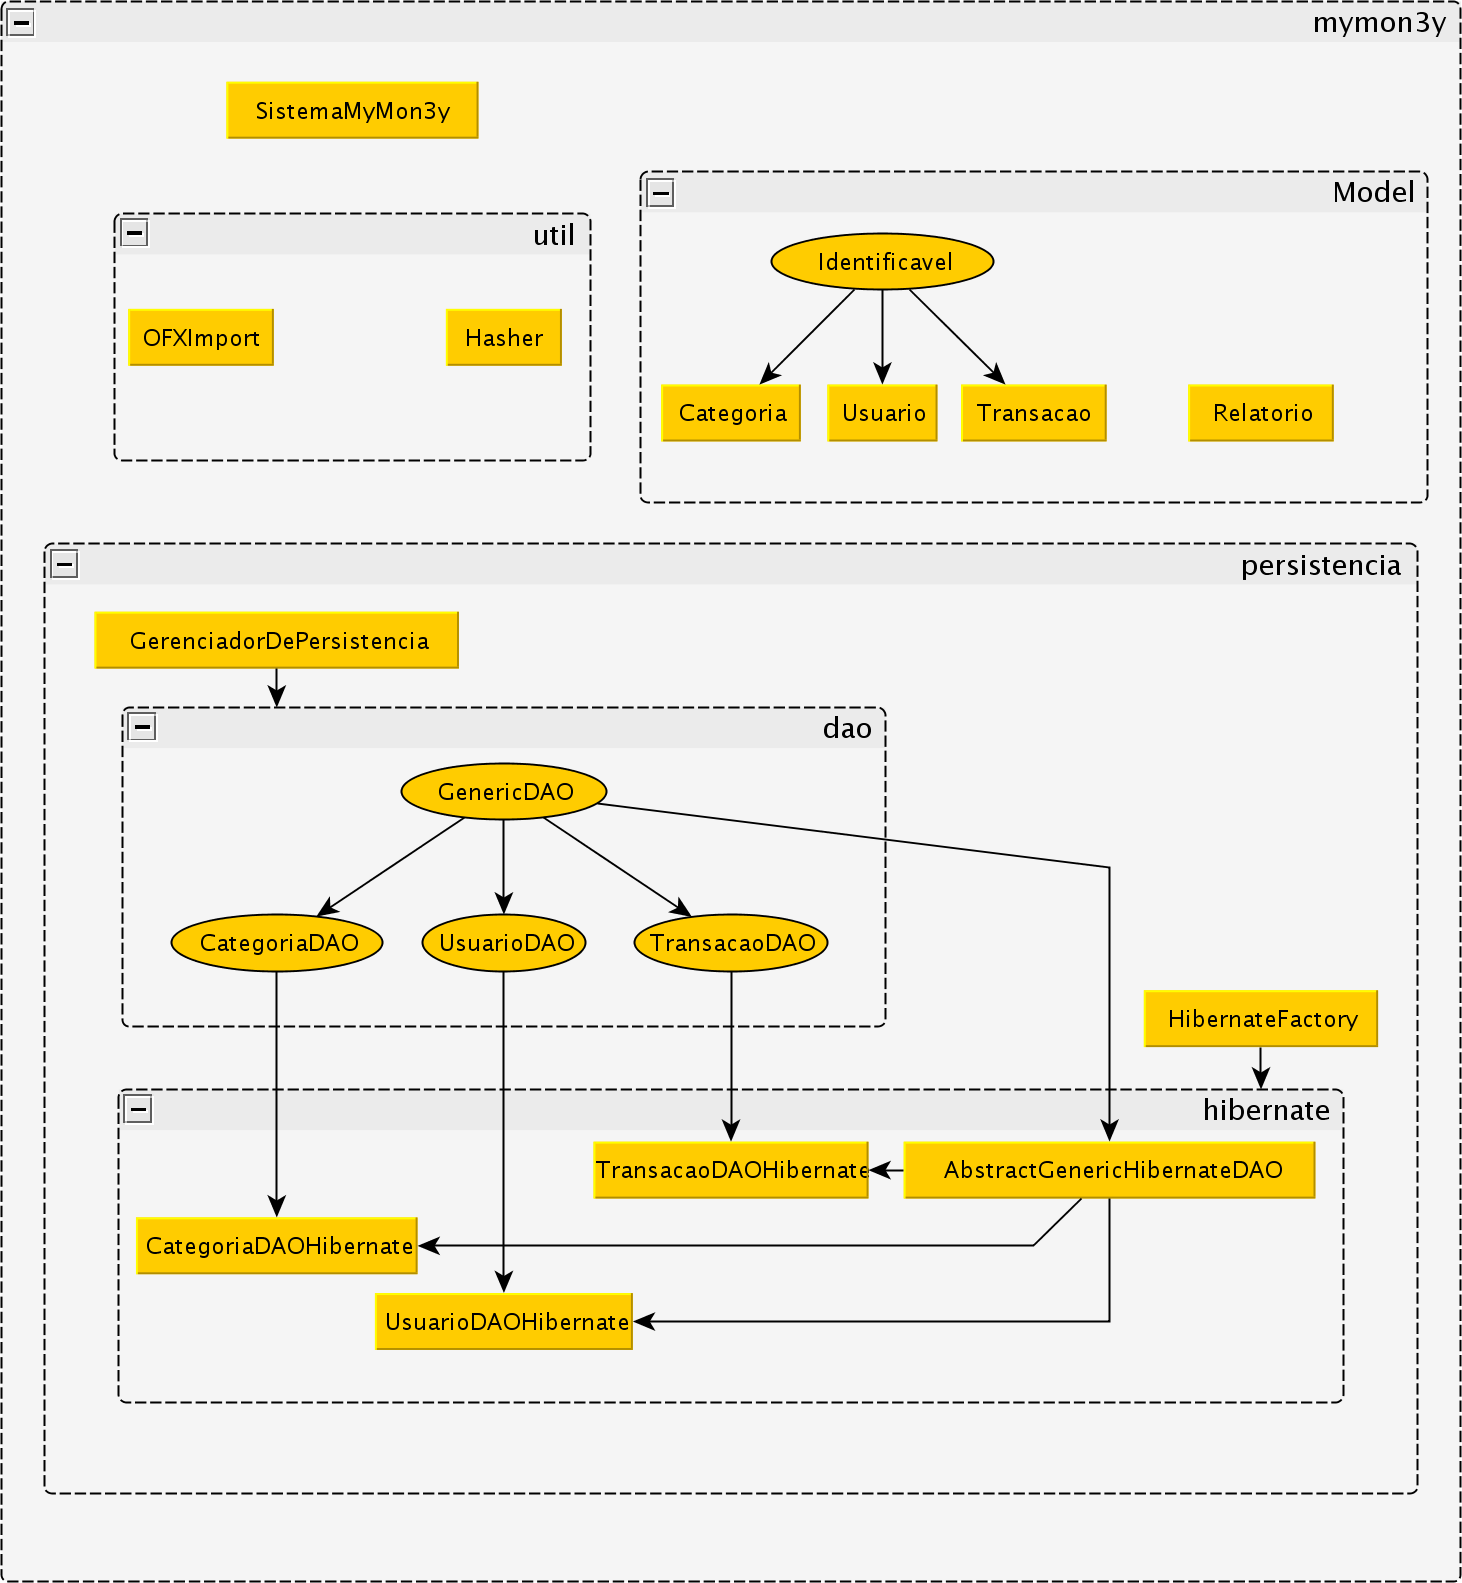
\includegraphics[scale=0.2, bb=0 0 1462 1583]{arquitetura.png}
  % modelo.png: 449x1183 pixel, 72dpi, 15.84x41.73 cm, bb=0 0 449 1183
  \caption{Diagrama de Classes}
\end{figure}

A \textit{Facade} será utilizada em uma etapa posterior do projeto, estruturando o sistema através da arquitetura \textit{Model-View-Controller}\cite{MVC}. Nesta arquitetura, é clara a separação de uma lógica distinta para três entidades:

\begin{description}
 \item[Model] Implementa a lógica de negócio.
 \item[View] Trata da visualização da interface com o usuário.
 \item[Controller] Intermeia os pedidos oriundos da interface com o \textit{Model}; manipula o estado da sessão; e em alguns casos, prepara o Model para ser entregue a \textit{View}.
 \end{description}

\section{Tecnologias e Implementação}
\label{tecnologias}

O projeto é desenvolvido em \textbf{Java} (1.6) utilizando o \textbf{Eclipse} como ambiente de desenvolvimento, o \textbf{SVN} oferecido pelo Google Code (\url{http://code.google.com/p/mymon3y}) como controle de versão e o \textbf{Ant} (1.7) como ferramenta de controle de construção do software.

Para dar suporte ao uso de testes de aceitação, utiliza-se a biblioteca \textbf{EasyAccept}. Para a persistência das entidades de dados, utiliza-se o \textbf{Hibernate} (3.0), que realiza o mapeamento de objetos Java a um banco de dados. O \textbf{Hibernate} é capaz de realizar tal mapeamento para diversos banco de dados, o sistema faz uso do \textbf{Apache Derby} (10.4) como o banco de dados utilizado. Esta escolha é motivada pela capacidade de funcionamento embarcado desta base de dados, permitindo que o ambiente de testes seja facilmente criado sem a necessidade de gerenciar ou ativar um serviço externo.

%\bibliographystyle{sbc}
%\bibliography{psoo}

\end{document}
